\section{Addition}
\paragraph{Study1}
%To further observe the influence of uplift events for students facing stressor events,
%we statistic all the stressful intervals~\cite{Li2017Analyzing} detected surround the scheduled examinations over the 124 students during their high school career.
%For each student, we divide all his/her stressful intervals into two sets:
%1) stressful intervals under the influence of neighbouring uplift events (e.g., \emph{Halloween activity}), and 2) independent stressful intervals.
%Figure~\ref{fig:frequency} shows five measures of each student during the above two conditions:
%the \emph{accumulated stress}, the \emph{average stress} (per day), the \emph{length of stressful intervals},
%the \emph{frequency of academic topic words}, and the \emph{ratio of academic stress among all types of stress}.
%For each measure, we calculate the average value over all eligible slides for each student.
%\begin{figure}
%\centering
%\caption{Compare students' stress during exam intervals in two situations:
%1) affected by neighboring uplift events (U-SI), 2) no uplift events occurred nearby (SI)}
%\includegraphics[width=\linewidth]{figs/frequency.eps}
%\label{fig:frequency}
%\end{figure}

\linespread{1.1}
\begin{table}[H]
\begin{center}
\caption{\small{Structured extraction of positive events from microblogs.}}
\small{
\begin{tabular}{l} \hline \rowcolor{gray!40}
I am really looking forward to the spring outing on Sunday now. \\ \rowcolor{gray!40}
(Doer:\emph{I}, Act:\emph{looking forward}, Object:\emph{spring outing})\\
My holiday is finally coming [smile]. \\
(Doer:\emph{My holiday}, Act:\emph{coming}, Object:\emph{[smile]})\\ \rowcolor{gray!40}%\hline
First place in my lovely math exam!!! In memory of it.\\ \rowcolor{gray!40}
Object:\emph{first place, math, exam, memory})\\ %\hline
You are always here for me like sunshine. \\
(Doer:\emph{You}, Object:\emph{sunshine})\\ \rowcolor{gray!40} %\hline
Thanks all my dear friends to take the party for me. Happiest birthday!\\ \rowcolor{gray!40}
(Doer:\emph{friends}, Act:\emph{thanks}, Object:\emph{party, birthday})\\
%Be yourself. Trust yourself and follow your heart. \\
%(Doer:\emph{yourself}, Act:\emph{trust}, Object:\emph{heart})\\ \rowcolor{gray!40} %\hline
%Feel proud of our play in the Games. Our class is always the family!!!\\ \rowcolor{gray!40}
%(Doer:\emph{Our}, Object:\emph{class, family})\\
%A good film always makes bring comfort and happiness to me.\\
%(Doer:\emph{me}, Act:\emph{bring}, Object:\emph{comfort, happiness})\\ \rowcolor{gray!40}%\hline
I know my mom is the one who support me forever, no matter \\ %\rowcolor{gray!40}
when and where. (Doer:\emph{mom}, Act:\emph{support})\\ \hline
\end{tabular}}
\label{tab:uplifts}
\end{center}
\end{table}

\linespread{1.1}
\begin{table}[H]
\begin{center}
\caption{\small{Structured extraction of stressor events from microblogs.}}
\small{
\begin{tabular}{l} \hline \rowcolor{gray!40}
I don't know how long can I bear the nag.\\ \rowcolor{gray!40}
(Doer:\emph{I}, Act:\emph{bear}, Object:\emph{nag})\\ %\hline
Parents like to judge everything around me with their emotion.
\\(Doer:\emph{parents}, Act:\emph{judge}, Object:\emph{everything})\\ \rowcolor{gray!40}
%Hope that my mother could revive earlier.\\ \rowcolor{gray!40}
%(Doer:\emph{my mother}, Act:\emph{revive})\\%\hline
Every one betrayed me. \\ \rowcolor{gray!40}
(Doer:\emph{every one}, Act:\emph{betray}, Object:\emph{me})\\ \hline
I'm too weak to handle such a fierce competition.\\ %\rowcolor{gray!40}
(Doer:\emph{I}, Act:\emph{too weak to handle}, Object:\emph{competition})\\ \rowcolor{gray!40}
%I just felt hurt, depressed, self-abased and sad.
%\\(Doer:\emph{I}, Act:\emph{feel hurt, depressed, self-abased and sad})\\ \rowcolor{gray!40}%\hline
%My holiday is filled with all kinds of homework.\\ \rowcolor{gray!40}
%(Doer:\emph{My holiday}, Act:\emph{fill with}, Object:\emph{homework})\\ %\hline
%Unescapably, it's time to go back to school.
%\\(Act:\emph{go back}, Object:\emph{school})\\ \rowcolor{gray!40} %\hline
When can you be aware of my heart-broken feeling again and again?\\ \rowcolor{gray!40}
(Doer:\emph{you}, Act:\emph{be aware of}, Object:\emph{heart-broken feeling})\\ \hline
\end{tabular}
}
\label{tab:stressors}
\end{center}
\end{table}